
\section{Resultados}

\subsection{Red de interacción entre genes}

Se identificaron un total de 51 genes asociados al fenotipo \textbf{Papilloma} y obtuvimos una representación visual de la red de interacción entre los genes.


\subsection{Análisis de enriquecimiento funcional}

Se realizó un análisis de enriquecimiento funcional destacando las categorías \textbf{Process} y \textbf{KEGG}, obteniendo relaciones entre algunos grupos de genes con problemas del sistema inmune, carcinoma y las adipoquinas.

Los términos y categorías relacionados con enfermedades como \textbf{cervix}, \textbf{ovarian}, \textbf{HPV}, \textbf{herpes}, \textbf{papillomavirus}, \textbf{costellos} y \textbf{cowden} fueron encontrados en el análisis de enriquecimiento funcional, indicando posibles vínculos entre estos términos y los genes asociados al fenotipo estudiado.

Se realizaron búsquedas específicas de genes clave como \textit{TP53}, \textit{AKT1}, \textit{SDHB}, \textit{SDHD}, \textit{HRAS} dentro de las categorías significativas. Estos genes podrían tener una importancia particular en relación con el fenotipo de interés, evidenciando su posible relevancia funcional.

\subsection{Descarga y procesamiento de la red de interacción}

Se descargó la red de interacción en formato TSV. El archivo descargado se procesó para dar como resultado un archivo de texto \textbf{$genes_igraph.txt$} formado por dos columnas de nombres de genes, en las que cada fila representa una relación entre dos genes.



\subsection{Propiedades de la red y detección de comunidades}

En nuestra red vimos que todos los nodos estaban conectados entre sí y que se trataba de un grafo no dirigido.

\vspace{3pt}

Obtuvimos una tabla con el \textbf{grado de centralidad} de cada gen (tabla \ref{tab:gradoCentralidad}). Pudimos observar como el gen de interés \textit{TP53} es el que presentaba un mayor grado de centralidad y por tanto más relaciones con otros genes. 



	\begin{table}[h]
		\begin{minipage}{0.5\textwidth}
			\centering
			\begin{tabular}{|c|c|}
				\hline
				Gen & Grado Centralidad\\
				\hline
				CD4 & 15\\
				\hline
				CD79A & 13 \\
				\hline
				SPL1 & 11 \\
				\hline
				DDB2 & 9 \\
				\hline
				LRRC8A & 4 \\
				\hline
				FLT4 & 5 \\
				\hline
				TCF3 & 10 \\
				\hline
				IL7 & 10 \\
				\hline
				PIK3CA & 11 \\
				\hline
				MSH3 & 11 \\
				\hline
				TP53 & 30 \\
				\hline
				XPC & 9 \\
				\hline
				ERCC3 & 9 \\
				\hline
				ERCC4 & 9 \\
				\hline
				USF3 & 1 \\
				\hline
				TMC8 & 5 \\
				\hline
				IGLL1 & 7 \\
				\hline
				CARMIL2 & 1 \\
				\hline
				SEC23B & 2 \\
				\hline
				GATA2 & 10 \\
				\hline
				SASH3 & 3 \\
				\hline
			\end{tabular}
			\vspace{3pt}
			\caption{Grado Centralidad}
			\label{tab:gradoCentralidad}
		\end{minipage}%
		\begin{minipage}{0.5\textwidth}
			\centering
			\begin{tabular}{|c|c|}
				\hline
				Gen & Grado Centralidad \\
				\hline
				SDHC & 5\\
				\hline
				NRAS & 8 \\
				\hline
				PTEN & 15 \\
				\hline
				STK4 & 2 \\
				\hline
				XPA & 9 \\
				\hline
				SDHB & 7 \\
				\hline
				SDHD & 5 \\
				\hline
				TPP2 & 2 \\
				\hline
				DCLRE1C & 10 \\
				\hline
				RHOH & 8 \\
				\hline
				ERCC2 & 8 \\
				\hline
				CD79B & 11 \\
				\hline
				CXCR4 & 12 \\
				\hline
				HRAS & 9 \\
				\hline
				PIK3R1 & 12 \\
				\hline
				AKT1 & 20 \\
				\hline
				TMC6 & 4 \\
				\hline
				IKBKG & 4 \\
				\hline
				DOCK8 & 7 \\
				\hline
				ERCC5 & 9 \\
				\hline
			\end{tabular}
			
			
		\end{minipage}
	\end{table}
	



\vspace{3pt}

En cuanto al \textbf{grado de conectividad} obtuvimos un valor del 19\%, el cual era bastante pequeño y nos indicaba que nuestro grafo no era muy fuerte. Esto puede deberse a que las comunidades entre si no tenían una gran dependencia y teníamos varios genes que no nos interesaban. 

\vspace{3pt}

Empleamos distintos algoritmos para \textbf{detectar comunidades}. En el caso del método de Girvan-Newman había nodos que no pertenecían a ninguna comunidad (Fig. \ref{fig:algoritmos}-A). Esto podía deberse a la forma en que el algoritmo de betweenness identifica comunidades. Puede detectar comunidades basándose en la centralidad de intermediación de los nodos, y algunos nodos pueden no estar claramente vinculados a una comunidad en función de esta medida.

\vspace{3pt}

Con el algoritmo voraz vimos que nuestros genes de interés se encontraban en el mismo cluster de color amarillo (\textit{TP53}, \textit{AKT1}, \textit{SDHB}, \textit{SDHD}, \textit{HRAS}). Además, todos los nodos pertenecían a alguna comunidad (Fig. \ref{fig:algoritmos}-B), al igual que con el algoritmo de propagación de etiquetas (Fig. \ref{fig:algoritmos}-C). Sin embargo, en este último obtuvimos tan solo 3 comunidades por lo que la clusterización es mínima.  Con la aplicación del método de Louvain también resultaban menos comunidades que con el algoritmo voraz. Observamos 4 comunidades (Fig. \ref{fig:algoritmos}-D). 

\begin{figure}
	\centering
	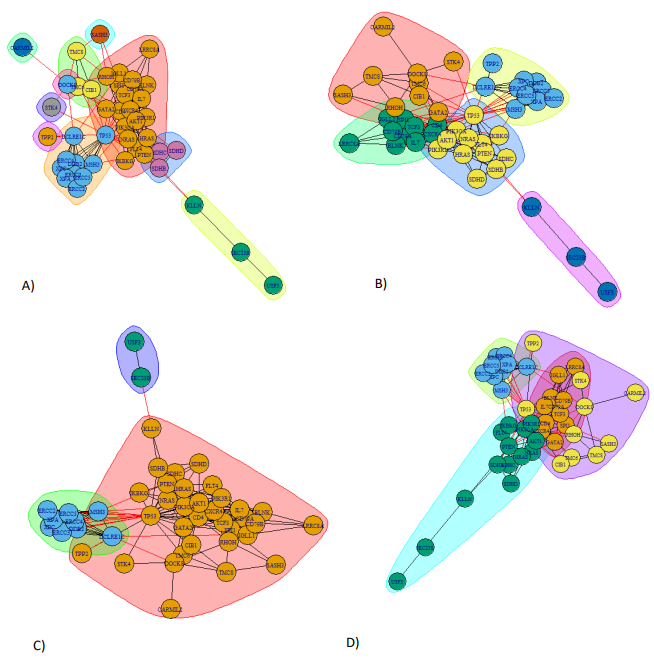
\includegraphics[width=0.98\linewidth]{figures/algoritmos}
	\captionsetup{labelformat=empty}
	\caption{Resultado de la aplicación de distintos algoritmos de clusterización a la red. Figura A) algoritmo de Girvan-Newman. Figura B) algoritmo voraz. Figura C) método de propagación de etiquetas. FIgura D) algoritmo de Louvain}
	\label{fig:algoritmos}
\end{figure} 



Los algoritmos anteriores tenían la desventaja de que no reflejaban con exactitud la posibilidad de que un gen perteneciera a más de una comunidad. Para estudiar esto hicimos uso de \textbf{Link Communities}, y obtuvimos una gráfica donde cada gen era representado por un diagrama de sectores (Fig. \ref{fig:link}). Observamos que la mayoría de los genes pertenecen a más de una comunidad. Al centrarnos en nuestros genes de interés detectamos que el gen \textit{TP53} tenía relación con 4 clusters distintos mientras que los otros genes de interés, \textit{SDHB}, \textit{SDHb},\textit{HRAS}, \textit{AKT1} se encontraban en una comunidad más diferenciada de color rosa. 

\begin{figure}
	\centering
	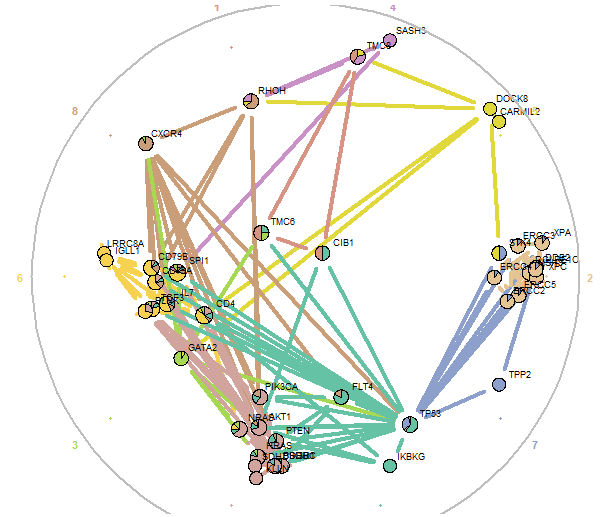
\includegraphics[width=0.8\linewidth]{figures/link}
	\caption{Resultado de la aplicación de detección de comunidades mediante link communities.}
	\label{fig:link}
\end{figure}



Para el \textbf{estudio genes de interés} obtuvimos la tabla \ref{tab:genesinteres} con el gen en concreto y sus genes vecinos. Observamos que todos los genes estaban relacionados entre sí menos el caso de \textit{TP53} y \textit{SDHD}. 

\begin{table}[h]
	\centering
	\caption{Genes de interes y genes relacionados}
	\begin{tabular}{|c|c|}
		\hline
		\textbf{Genes} & \textbf{Genes interes} \\
		\hline
		TP53 & SDHB,HRAS,AKT1 \\
		\hline
		HRAS & TP53,SDHB,SDHS,AKT1 \\
		\hline
		AKT1 & TP53,SDHB,SDHD,HRAS \\
		\hline
		SDHB & TP53,SDHD,HRAS,AKT1 \\
		\hline
		SDHD & SDHB,HRAS,AKT1 \\
		\hline
	\end{tabular}
	\label{tab:genesinteres}
\end{table}

\clearpage

\subsection{Relación de los genes de interés con fenotipos patológicos.}

Tras enriquecer el conjunto de genes de interés obtuvimos 729 entradas en las cuales encontramos relaciones de genes asociados con fenotipos patológicos que calificamos en estas tablas \ref{palabra-clave-papiloma}, \ref{palabra-clave-genital}, \ref{palabra-clave-renal}, \ref{palabra-clave-carcinoma}, \ref{palabra-clave-ovario}, \ref{palabra-clave-utero}, según la palabra clave por la cual buscamos:

\begin{table}[h]
	\centering
	\caption{Fenotipos patológicos con palabra clave papiloma}
	\begin{tabular}{|p{6cm}|p{6cm}|}
		\hline
		\textbf{Genes} & \textbf{Fenotipos patológicos asociados} \\
		\hline
		FLT4, PIK3CA, TP53, SDHC, NRAS, PTEN, SDHB, SDHD, HRAS, PIK3R1, AKT1, IKBKG & Papiloma \\
		\hline
		TP53, NRAS & Papiloma del plexo coroideo \\
		\hline
	\end{tabular}
	\label{palabra-clave-papiloma}
\end{table}

\begin{table}[h]
	\centering
	\caption{Fenotipos patológicos con palabra clave genital}
	\begin{tabular}{|p{6cm}|p{6cm}|}
		\hline
		\textbf{Genes} & \textbf{Fenotipos patológicos asociados} \\
		\hline
		PIK3CA, TP53, SDHC, NRAS, PTEN, SDHB, SDHD, AKT1 & Neoplasia genital \\
		\hline
		FLT4, PIK3CA, TP53, SDHC, NRAS, PTEN, SDHB, SDHD, HRAS, AKT1 & Anomalía de los genitales externos masculinos \\
		\hline
		PIK3CA, TP53, SDHC, NRAS, PTEN, SDHB, SDHD, AKT1 & Morfología anormal de los genitales internos femeninos \\
		\hline
	\end{tabular}
	\label{palabra-clave-genital}
\end{table}

\begin{table}[h]
	\centering
	\caption{Fenotipos patológicos con palabra clave renal}
	\begin{tabular}{|p{6cm}|p{6cm}|}
		\hline
		\textbf{Genes} & \textbf{Fenotipos patológicos asociados} \\
		\hline
		PIK3CA, TP53, SDHC, NRAS, PTEN, SDHB, SDHD, AKT1 & Neoplasia renal \\
		\hline
		PIK3CA, SDHC, NRAS, PTEN, SDHB, SDHD, AKT1 & Carcinoma de células renales \\
		\hline
		PIK3CA, TP53, SDHC, PTEN, SDHB, SDHD, AKT1 & Anomalía de las glándulas suprarrenales \\
		\hline
		TP53, SDHC, PTEN, SDHB, SDHD & Neoplasia de la glándula suprarrenal \\
		\hline
		SDHC, SDHB, SDHD & Feocromocitoma extraadrenal \\
		\hline
		SDHC, SDHB, SDHD & Feocromocitoma suprarrenal \\
		\hline
	\end{tabular}
	\label{palabra-clave-renal}
\end{table}

\begin{table}[h]
	\centering
	\caption{Fenotipos patológicos con palabra clave carcinoma}
	\begin{tabular}{|p{6cm}|p{6cm}|}
		\hline
		\textbf{Genes} & \textbf{Fenotipos patológicos asociados} \\
		\hline
		PIK3CA, SDHC, NRAS, PTEN, SDHB, SDHD, HRAS, AKT1 & Carcinoma folicular de tiroides \\
		\hline
		PIK3CA, TP53, SDHC, NRAS, PTEN, SDHB, SDHD, HRAS, AKT1 & Carcinoma de tiroides \\
		\hline
		PIK3CA, TP53, SDHC, PTEN, SDHB, SDHD, AKT1 & Carcinoma de mama \\
		\hline
		PIK3CA, SDHC, NRAS, PTEN, SDHB, SDHD, AKT1 & Carcinoma de células renales \\
		\hline
		PIK3CA, SDHC, PTEN, SDHB, SDHD, AKT1 & Carcinoma de endometrio \\
		\hline
		PIK3CA, NRAS, PTEN, HRAS, AKT1 & Carcinoma de células transicionales de vejiga \\
		\hline
		PIK3CA, NRAS, AKT1 & Carcinoma colorrectal hereditario no polipósico \\
		\hline
		NRAS, HRAS1 & Carcinoma no medular de tiroides \\
		\hline
		PIK3CA, AKT1 & Adenocarcinoma papilar de ovario \\
		\hline
		PIK3CA, TP53 & Adenocarcinoma de pulmón \\
		\hline
		NRAS, HRAS & Carcinoma papilar de tiroides \\
		\hline
		NRAS, HRAS & Carcinoma basocelular \\
		\hline
		PIK3CA, TP53 & Carcinoma hepatocelular \\
		\hline
		TP53, AKT1 & Carcinoma \\
		\hline
	\end{tabular}
	\label{palabra-clave-carcinoma}
\end{table}

\begin{table}[h]
	\centering
	\caption{Fenotipos patológicos con palabra clave ovario y derivados}
	\begin{tabular}{|p{6cm}|p{6cm}|}
		\hline
		\textbf{Genes} & \textbf{Fenotipos patológicos asociados} \\
		\hline
		PIK3CA, TP53, PTEN, AKT1 & Neoplasia ovárica \\
		\hline
		PIK3CA, AKT1 & Adenocarcinoma papilar de ovario \\
		\hline
		PIK3CA, TP53, SDHC, PTEN, SDHB, SDHD, AKT1 & Anomalía del ovario \\
		\hline
		PIK3CA, SDHC, PTEN, SDHB, SDHD, AKT1 & Ovarios poliquísticos agrandados \\
		\hline
	\end{tabular}
	\label{palabra-clave-ovario}
\end{table}

\begin{table}[h]
	\centering
	\caption{Fenotipos patológicos con palabra clave útero y derivados}
	\begin{tabular}{|p{6cm}|p{6cm}|}
		\hline
		\textbf{Genes} & \textbf{Fenotipos patológicos asociados} \\
		\hline
		PIK3CA, SDHC, NRAS, PTEN, SDHB, SDHD, AKT1 & Neoplasia uterina \\
		\hline
		PIK3CA, NRAS, AKT1 & Leiomiosarcoma uterino \\
		\hline
		FLT4, SDHB, SDHD, PIK3R1 & Retraso del crecimiento intrauterino \\
		\hline
	\end{tabular}
	\label{palabra-clave-utero}
\end{table}
\clearpage
